\begin{figure*}[!t]
        \centering{
                \begin{tabular}{cccccc}
                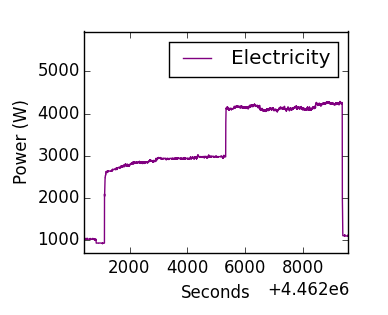
\includegraphics[width=2.1in]{multidisaggfig/heatingIndoorOutdoorPattern1_sum.png}&
                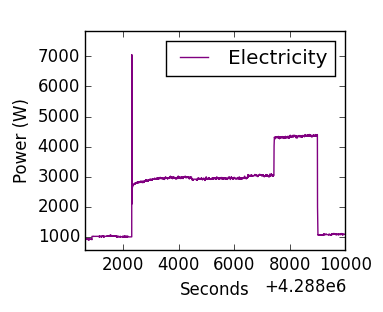
\includegraphics[width=2.1in]{multidisaggfig/heatingIndoorOutdoorPattern2_sum.png}&
                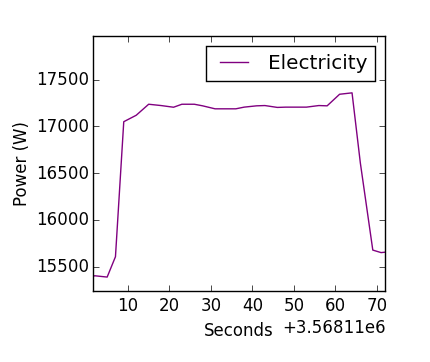
\includegraphics[width=2.1in]{multidisaggfig/microwave_sum.png}\tabularnewline
                (a) & (b)&(c)\tabularnewline
                 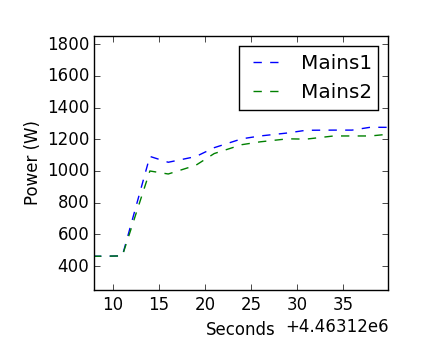
\includegraphics[width=2.1in]{multidisaggfig/heatingIndoorOutdoorPattern1.png}&
                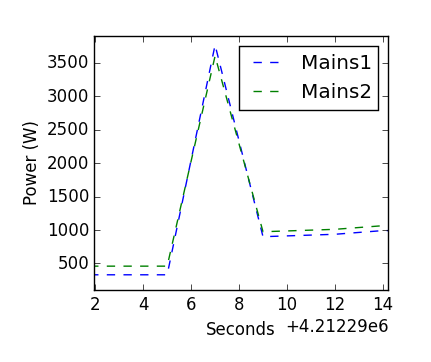
\includegraphics[width=2.1in]{multidisaggfig/heatingIndoorOutdoorPattern2.png}&
                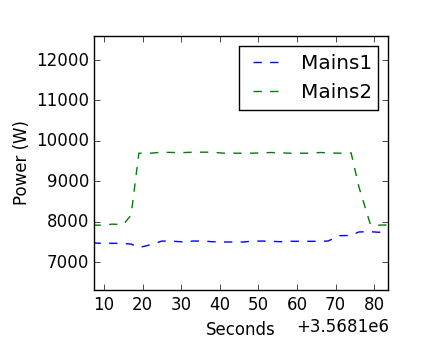
\includegraphics[width=2.1in]{multidisaggfig/microwave.png}\tabularnewline
                (d) & (e)&(f)\tabularnewline
                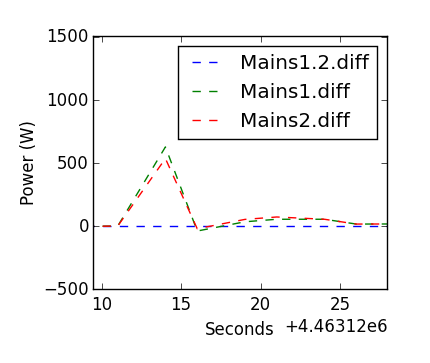
\includegraphics[width=2.1in]{multidisaggfig/heatingIndoorOutdoorPhase12On_1.png}&
                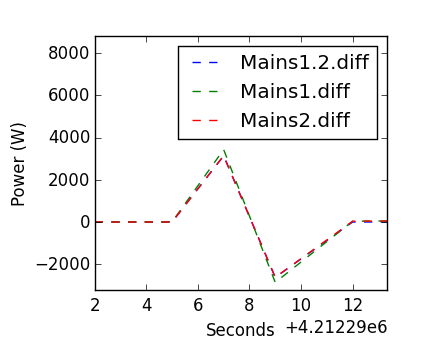
\includegraphics[width=2.1in]{multidisaggfig/heatingIndoorOutdoorPhase12On_2.png}&
                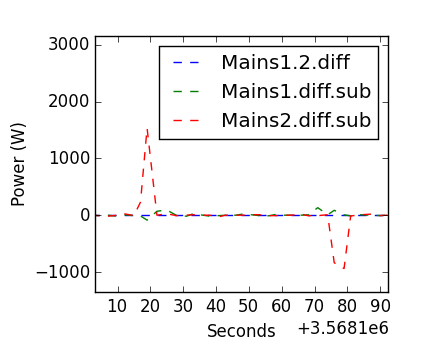
\includegraphics[width=2.1in]{multidisaggfig/microwavePhase2OnOff.png}\tabularnewline
               (g)&(h)&(i)\tabularnewline
                \end{tabular}
                }
        \caption{
       Devices (a) heatingIndoorOutdoor (b) heatingIndoorOutdoor (another pattern) (c) microwave in the aggregated power of sum of mains1 and main2. 
       Devices (d) heatingIndoorOutdoor (e) heatingIndoorOutdoor (another pattern) (f) microwave in the aggregated power of mains1 and main2. 
       Devices (g) heatingIndoorOutdoor (h) heatingIndoorOutdoor (another pattern) (i) microwave in the diffs data of aggregated power of mains1 and main2. 
       Since all of them starts synchronously in two mains, they are disaggregated by multivariate piecewise motif mining.  
}
        \label{fig_patterns}
\end{figure*}